\begin{frame}{Optimization}
\begin{itemize}
    \item We know how to represent our logistic and linear regression functions:
    $$y =(w_0 + w_1x_1 + ... + w_Dx_D)$$
    $$y = \sigma(w_0 + w_1x_1 + ... + w_Dx_D)$$
    \item We need some algorithm for finding what the best choices of $(w_0, ..., w_D)$ are.
    \item \textbf{Gradient Descent} is a process by which we iteratively improve our choices for $(w_0, ..., w_D)$ by computing the \textbf{gradient} of the \textbf{loss} of our predictions.
\end{itemize}
\end{frame}

\begin{frame}{Optimization}
\begin{itemize}
    \item \textbf{Gradients} equal the slope of the line that is \textit{tangent} to your function.
    \item Imagine that one of these lines exists for each point along your function.
    \begin{figure}
    \centering
    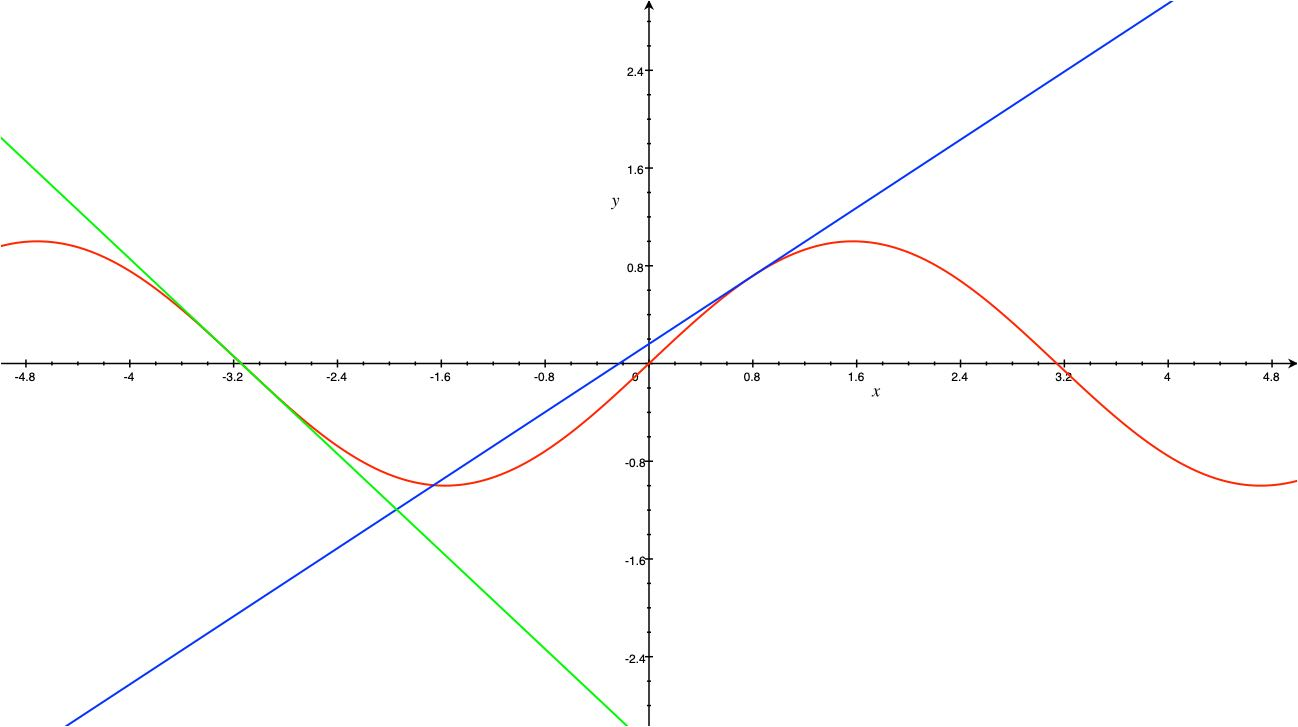
\includegraphics[width=0.6\textwidth]{img/TwoTangentLine.jpg}
    \caption{Lines tangent to $y = sin(x)$ at $x = 0.8$ and $x=-3.2$}
    \end{figure}
    \item They indicate the direction in which the function is increasing.
    
\end{itemize}
\end{frame}

\begin{frame}{Optimization}
    \begin{center}
    \item Physical Metaphor: The function is a hill. A \textbf{positive} gradient indicates a ball would roll \textbf{left}, a negative gradient indicates a \textbf{ball} would roll \textbf{right}.
    \end{center}
\end{frame}

\begin{frame}{Optimization}
\begin{itemize}
    \item A common loss function is the \textbf{Mean Squared Error} $\mathcal{L}(y, \hat{y}) = (y - \hat{y})^2$. Why do you think that is?
\end{itemize}
\end{frame}

\begin{frame}{Optimization}
\begin{itemize}
    \item A common loss function is the \textbf{Mean Squared Error} $\mathcal{L}(y, \hat{y}) = (y - \hat{y})^2$. Why do you think that is?
    \begin{figure}
    \centering
    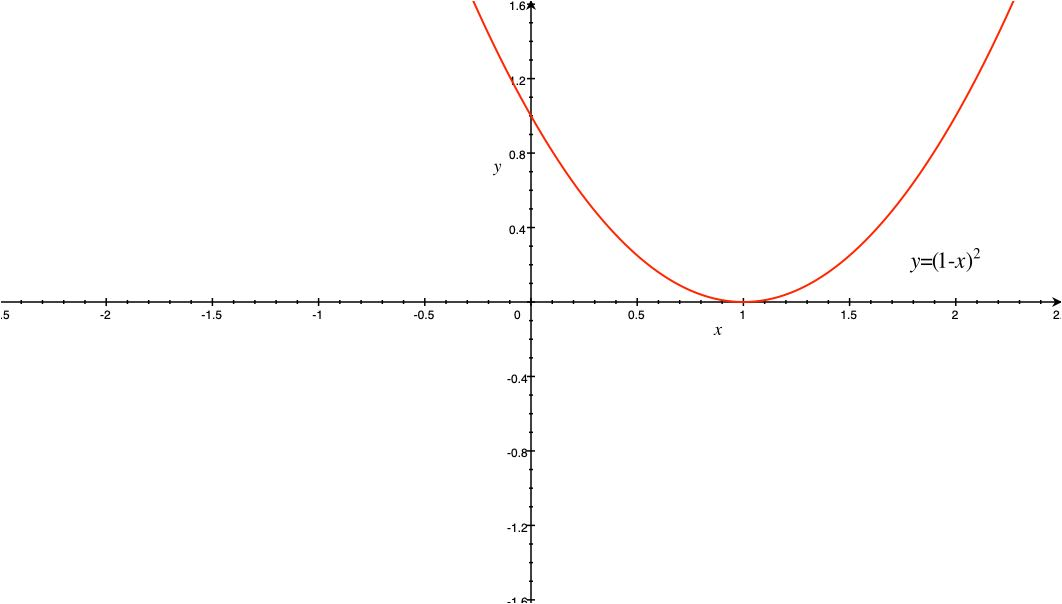
\includegraphics[width=0.6\textwidth]{img/MSELoss.jpg}
    \caption{Graph of $y=(1-x)^2$}
    \end{figure}
\end{itemize}
\end{frame}

\begin{frame}{Optimization}
    \begin{figure}
    \centering
    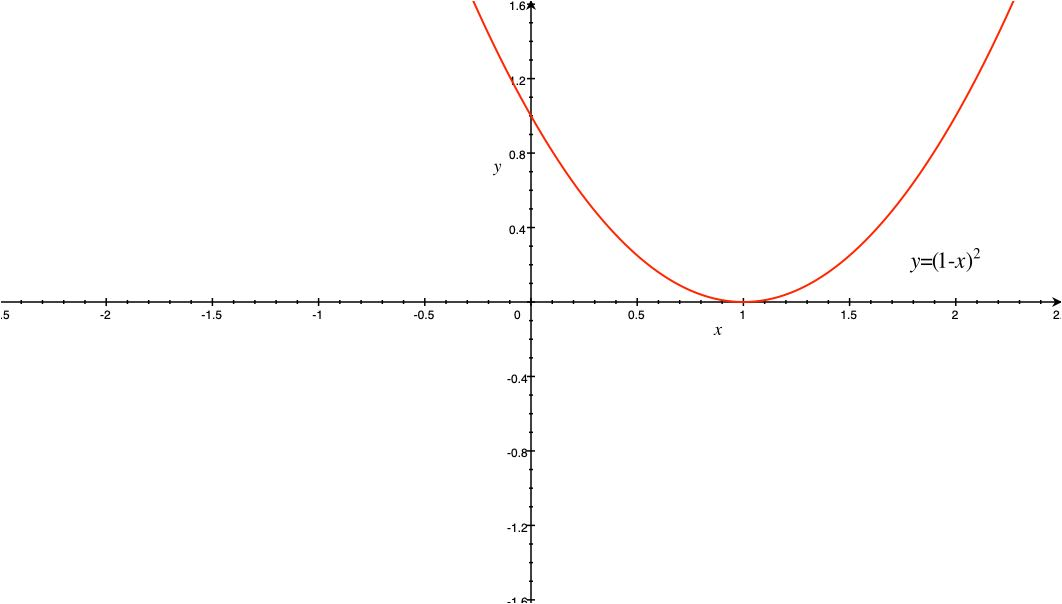
\includegraphics[width=0.8\textwidth]{img/MSELoss.jpg}
    \caption{Graph of $y=(1-x)^2$} or $\mathcal{L}(y=1, \hat{y}) = (1-\hat{y})^2$
    \end{figure}
\end{frame}

\begin{frame}{Optimization}
\begin{itemize}
    \item \textbf{Mean Squared Error} (MSE) defined by $\mathcal{L}(y, \hat{y}) = (y - \hat{y})^2$. 
    \item What is $\hat{y}$? Its the output of linear or logistic regression!
    $$\hat{y} =(w_0 + w_1x_1 + ... + w_Dx_D)$$
    $$\hat{y} = \sigma(w_0 + w_1x_1 + ... + w_Dx_D)$$
    \item $y$ is the corresponding label to datapoint $(x_1, x_2, ..., x_D)$!
\end{itemize}
\end{frame}

\begin{frame}{Optimization}
    \begin{itemize}
        \item Collect a dataset of $(y, x_1, x_2, ..., x_D)$ sequences.
        \item Choose some initial weights randomly, $(w_0, w_1, ..., w_D)$
    \end{itemize}
    \begin{algorithm}[H]
    \SetAlgoLined
     \While{loss is not absolute minimum}{
      find $\hat{y} = \sigma(w_0 + w_1x_1 + ... + w_Dx_D)$ for each $(y, x_1, x_2, ..., x_D)$\;
      compute MSE $\mathcal{L}(y, \hat{y}) = (y - \hat{y})^2$\;
      recompute weights using \textbf{gradient} of your loss (shows direction to nudge your weights)\;
     }
     \caption{Gradient Descent Algorithm for Binary Classification}
    \end{algorithm}
    % \textbf{Gradient Descent algorithm procedure}
    % \item 
    % \item Solve either logistic or linear regression
    % $$\hat{y} =(w_0 + w_1x_1 + ... + w_Dx_D)$$
    % $$\hat{y} = \sigma(w_0 + w_1x_1 + ... + w_Dx_D)$$
    % \item Compute MSE $\mathcal{L}(y, \hat{y}) = (y - \hat{y})^2$
    % \item 
    
% \end{itemize}
    
\end{frame}